\title{16-bit full adder}
\date{}
\author{
	\IEEEauthorblockN{Daniel Josué Rodríguez Agraz}
	\IEEEauthorblockA{
		\textit{Communications and Electronics Enginnering, Unniversidad de Guadalajara}\\
	}
}

\documentclass[conference]{IEEEtran}
\usepackage{filecontents,lipsum}
\usepackage[noadjust]{cite}
\usepackage{graphicx}
\usepackage{footmisc}
\usepackage{listings}
\usepackage{subcaption}
\usepackage{fancyhdr}
\usepackage{url}
\usepackage{hyperref}
\usepackage{array}
\usepackage{float}
\usepackage{adjustbox}
\usepackage{subcaption}
\hypersetup{
	colorlinks=true,
	linkcolor=black,
	urlcolor=blue,
	citecolor=black
}

\begin{document}
	
	\maketitle
	\begin{abstract}
		This document presents the design and verification process of a 16-bit full adder digital circuit. The design and verification were conducted using the SystemVerilog hardware description language, with simulation and compilation performed in Questasim software. Multiple instances of 1-bit, 2-bit, 4-bit, and 8-bit full adders were utilized to implement the 16-bit full adder design. Additionally, a test bench was developed to verify each instance and the final design, demonstrating the successful implementation of the circuit.
	\end{abstract}
	
	\section{Objectives}	
	The objective of this document is demonstrate the design, implementation, and operation of a 16-bit full adder. This includes detailing the underlying principles of binary addition, the structure and functionality of smaller adder units such as 1-bit, 2-bit, 4-bit, and 8-bit adders, and how they are interconnected to construct the 16-bit adder. Additionally, this document will cover the verification process used to ensure the correctness and efficiency of the design, highlighting both theoretical analysis and simulation results.
	\section{Introduction}
	
	A full adder is a fundamental digital circuit that performs the addition of two binary numbers, \( A \) and \( B \), along with a carry-in input \( C_{in} \). Figure \ref{fig:fa1b} illustrates the full adder, which has three inputs—\( A \), \( B \), and \( C_{in} \)—and two outputs—\( S \) (the sum) and \( C_{out} \) (the carry-out).
	
	\begin{figure}[H]
		\centering
		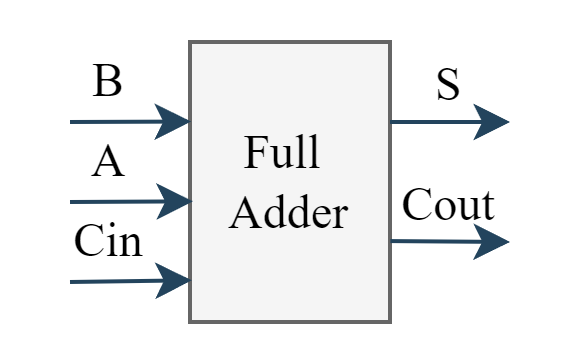
\includegraphics[width=0.6\columnwidth]{FA_1B}
		\caption{Logic symbol of a full adder.}
		\label{fig:fa1b}
	\end{figure}
	
	The full adder can be seen as a bit counter, where the output reflects the number of high-state inputs, as shown in the truth Table \ref{tab:full_adder_truth_table}. For example, with the combination \( A=0 \), \( B=0 \), and \( C_{in}=0 \), the outputs are \( C_{out}=0 \) and \( S=0 \), which can be interpreted as a logic 0. In contrast, for the combination \( A=0 \), \( B=1 \), and \( C_{in}=1 \), the outputs are \( C_{out}=1 \) and \( S=0 \), representing a binary 2, with \( C_{out} \) as the most significant bit (MSB) and \( S \) as the least significant bit (LSB). Furthermore, for the combination \( A=1 \), \( B=1 \), and \( C_{in}=1 \), the outputs are \( C_{out}=1 \) and \( S=1 \), which can be interpreted as a binary 3.
	
	\begin{table}[H]
		\centering
		\begin{tabular}{|m{.1cm}|m{0.2cm}|m{0.5cm}|m{0.5cm}|m{0.1cm}|}
			\hline
			\multicolumn{3}{|c|}{Inputs} & \multicolumn{2}{c|}{Outputs} \\
			\hline
			\(A\) & \(B\) & \(C_{in}\) & \(C_{out}\) & \(S\) \\
			\hline
			\(0\) & \centering\(0\) & \centering\(0\) & \centering\(0\) & \(0\) \\
			\(0\) & \centering\(0\) & \centering\(1\) & \centering\(0\) & \(1\) \\
			\(0\) & \centering\(1\) & \centering\(0\) & \centering\(0\) & \(1\) \\
			\(0\) & \centering\(1\) & \centering\(1\) & \centering\(1\) & \(0\) \\
			\(1\) & \centering\(0\) & \centering\(0\) & \centering\(0\) & \(1\) \\
			\(1\) & \centering\(0\) & \centering\(1\) & \centering\(1\) & \(0\) \\
			\(1\) & \centering\(1\) & \centering\(0\) & \centering\(1\) & \(0\) \\
			\(1\) & \centering\(1\) & \centering\(1\) & \centering\(1\) & \(1\) \\
			\hline
		\end{tabular}
		\caption{Truth table for a full adder.}
		\label{tab:full_adder_truth_table}
	\end{table}
	
	
	Two full adders can be connected in cascade to create a 2-bit full adder, as shown in Figure \ref{fig:fa2b}. In this circuit, there are still two inputs, \( A \) and \( B \), and two outputs, \( C_{out} \) and \( S \). The inputs \( A \) and \( B \), as well as the output \( S \), are 2-bit binary values. It should be noted that the input carry of the first full adder is fixed to zero, and the output carry is directly connected to the input carry of the next full adder.
	
	
	\begin{figure}[H]
		\centering
		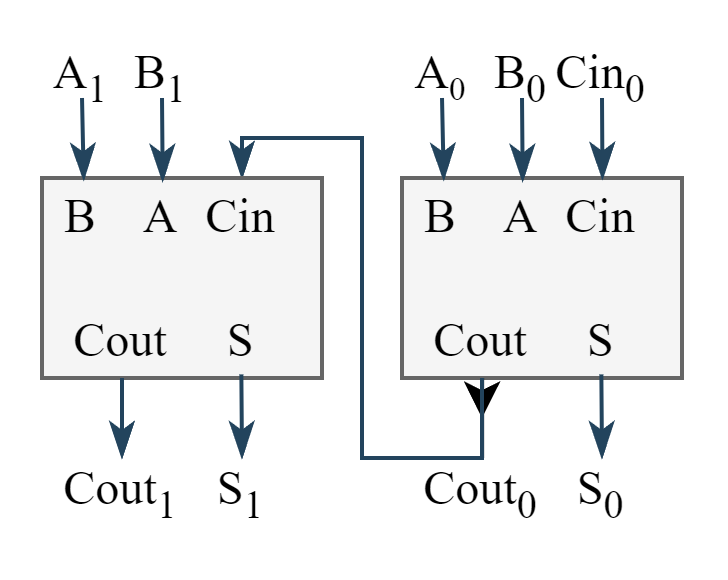
\includegraphics[width=0.6\columnwidth]{FA_2B}
		\caption{2 bit full adder.}
		\label{fig:fa2b}
	\end{figure}
	
	When adding 2 binary numbers they can be arranged like a usual decimal addition. For example when adding $101 + 011$, they can be rearranged like:
	\[	
	\begin{array}{c@{}c@{}c@{}c@{}}
		^1 & 1^1 & 0^1 & 1 \\ % Acarreos
		+ & 0 & 1 & 1  \\ % Números sumados
		\hline
		1 & 0 & 0 & 0  % Resultado
	\end{array}
	\]
	
	When there are at least two 1's, a carry is generated and propagates to the next digit. This carry bit is then added to the other digits in the following column.
	
	This methodology can be applied to n-bit adders. An n-bit adder can be constructed by cascading \(n\) full adders or by connecting multiple multi-bit full adders in series, like on the Figure \ref{fig:fanb}. For instance, we can cascade two 2-bit full adders to create a 4-bit adder, as shown in Figure \ref{fig:fa4b}, or connect two 4-bit full adders to form an 8-bit adder.
	
	\begin{figure}[H]
		\centering
		\begin{subfigure}[t]{\columnwidth}
			\centering
			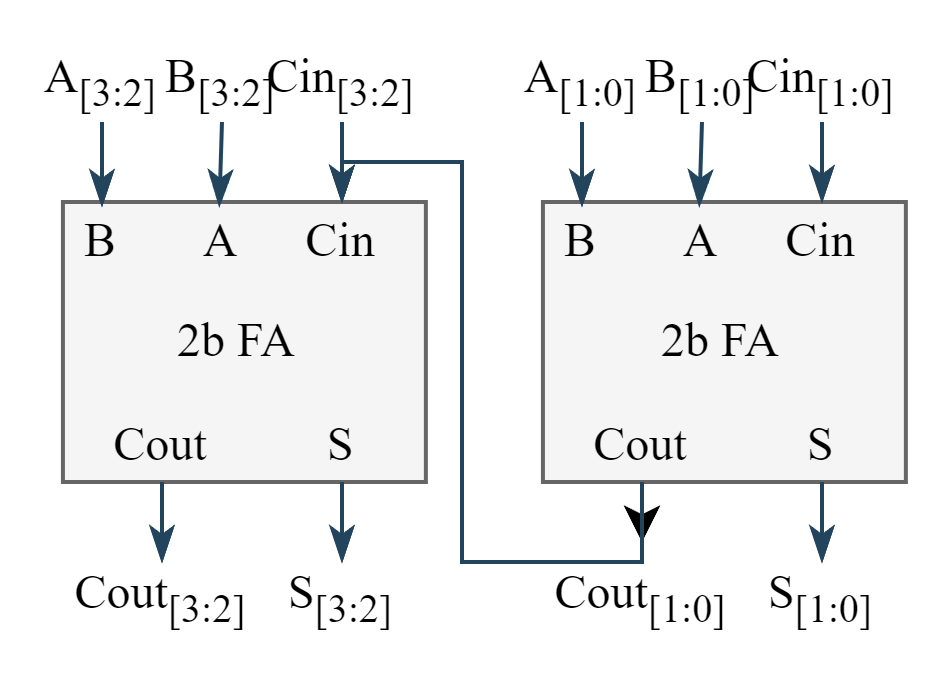
\includegraphics[width=0.7\columnwidth]{FA_4B}
			\caption{4-bit full adder made with two 2-bit full adders.}
			\label{fig:fa4b}
		\end{subfigure}
		~
		\begin{subfigure}[t]{\columnwidth}
			\centering
			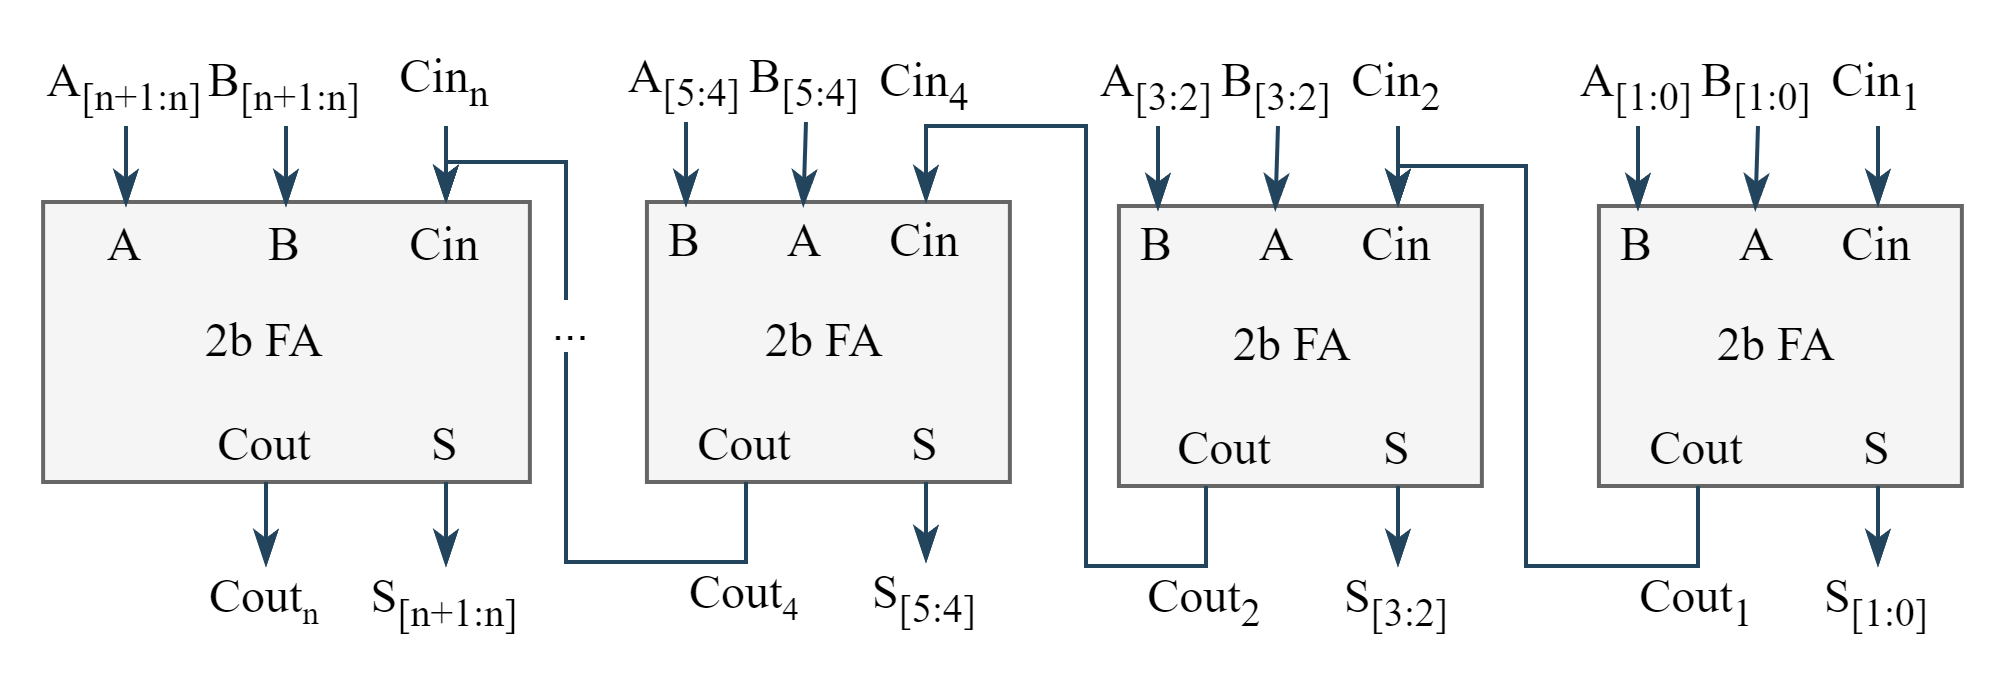
\includegraphics[width=\columnwidth]{FA_nB}
			\caption{n-bit full adder made with 2-bit full adders.}
			\label{fig:fanb}
		\end{subfigure}
		\caption{Comparison of full adders: \subref{fig:fa4b} shows a 4-bit full adder, while \subref{fig:fanb} illustrates an n-bit full adder.}
		\label{fig:2bfa_comp}
	\end{figure}
	
	
	\section{Methodology}
	This project was developed using SystemVerilog hardware description language, and it was compiled and simulated in Questasim software.
	
	To achieve this project we started designing a 1-bit full adder using Verilog, as shown in the code below. First, we had to define the amount of inputs and outputs of the project and the internal connections that would be. As shown in Figure \ref{fig:fa1b} we needed 3 inputs and 2 outputs.
	\begin{lstlisting}[language=Verilog, 
		caption={Full adder code hardware description in verilog.}, 
		label={code:FA_1B_Code}]
		module FA1
		(
		input wire A,B,Cin,
		output wire S, Cout
		);
		
		assign {Cout, S} = A + B + Cin;
		
		endmodule
		
	\end{lstlisting}
	
	After we made the 1-bi full adder, we wrote a test bench code with multiple cases to make sure the circuit worked as intended.
	
	\begin{lstlisting}[language=Verilog, 
		caption={Full adder code hardware description in verilog.}, 
		label={code:FA_1B_Code}]
		`timescale 1ns/1ps
		
		module FA1_tb;
		
		reg A;
		reg B;
		reg Cin;
		reg clk_tb;
		wire S;
		wire Cout;
		
		FA1 duv
		(
		.A(A),
		.B(B),
		.Cin(Cin),
		.S(S),
		.Cout(Cout)
		);
		
		initial
		begin
		clk_tb = 1'b0;
		A = 1'b0;
		B = 1'b0;
		Cin = 1'b0;
		#100;
		A = 1'b1;
		B = 1'b0;
		Cin = 1'b0;
		#100;
		A = 1'b0;
		B = 1'b1;
		Cin = 1'b0;
		#100;
		A = 1'b1;
		B = 1'b1;
		Cin = 1'b0;
		#100;*
		A = 1'b0;
		B = 1'b0;
		Cin = 1'b1;
		#100;
		A = 1'b1;
		B = 1'b0;
		Cin = 1'b1;
		#100;
		A = 1'b0;
		B = 1'b1;
		Cin = 1'b1;
		#100;
		A = 1'b1;
		B = 1'b1;
		Cin = 1'b1;
		#100;
		
		$stop;
		end
		
		always #10 clk_tb = !clk_tb;
		
		endmodule
		
	\end{lstlisting}
	
	As we did before, the first step is to determine the inputs and outputs of the circuit for a 2-bit full adder. As shown in Figure \ref{fig:fa2b}, a 2-bit full adder has three inputs: \( A \), \( B \), and \( C_{in} \), and two outputs: \( S \) and \( C_{out} \).
	
	Next, we need to define the internal connections. Specifically, the carry-out from the first adder must connect to the carry-in of the second adder. Finally, we instantiate the two full adders, assigning input variables appropriately. The first instance will receive the least significant bits (LSB) of \( A \) and \( B \), while the second instance will receive the most significant bits (MSB).
	
	Within the first adder, the carry-out is passed to an internal connection wire, which serves as the carry-in for the second adder. The output of the circuit will be a 2-bit result \( S \), with the carry-out \( C_{out} \) representing any overflow from the addition. The code below illustrates this process.
	
	\begin{lstlisting}[language=Verilog, 
		caption={2 bit full adder code hardware description in verilog.}, 
		label={code:FA_2B_Code}]
		`timescale 1ns/1ps
		
		module FA_2b
		(
		input wire A0,A1,B0,B1,Cin,
		output wire S0,S1,Cout1
		);
		
		wire carry;
		
		FA1 bit1
		(
		.A(A0),
		.B(B0),
		.Cin(Cin),
		.S(S0),
		.Cout(carry)
		);
		
		FA1 bit2
		(
		.A(A1),
		.B(B1),
		.Cin(carry),
		.S(S1),
		.Cout(Cout1)
		);
		
		endmodule
		
	\end{lstlisting}
	
	Finally, we create a test bench where all possible input cases are tested to ensure the desired output is obtained.\ref{}
	
	The last process will be repeated for the development of the 4,8 and 16-bit full adder.
	
	\section{Results}
	
	\subsection{Simulation results for the 1-bit full adder.}
	After coding the verification code, we test all of the cases defined on the test bench using the simulation tool of Questasim. Where we compare the results at the \(S\) and \(C_{out}\) output. On the Table \ref{tab:FA_1B_TT} the desired inputs and outputs are shown for a full adder.
	
	\begin{table}[H]
		\centering
		\begin{tabular}{|m{.1cm}|m{0.2cm}|m{0.5cm}|m{0.5cm}|m{0.1cm}|}
			\hline
			\multicolumn{3}{|c|}{Inputs} & \multicolumn{2}{c|}{Outputs} \\
			\hline
			\(A\) & \(B\) & \(C_{in}\) & \(C_{out}\) & \(S\) \\
			\hline
			\(0\) & \centering\(0\) & \centering\(0\) & \centering\(0\) & \(0\) \\
			\(0\) & \centering\(0\) & \centering\(1\) & \centering\(0\) & \(1\) \\
			\(0\) & \centering\(1\) & \centering\(0\) & \centering\(0\) & \(1\) \\
			\(0\) & \centering\(1\) & \centering\(1\) & \centering\(1\) & \(0\) \\
			\(1\) & \centering\(0\) & \centering\(0\) & \centering\(0\) & \(1\) \\
			\(1\) & \centering\(0\) & \centering\(1\) & \centering\(1\) & \(0\) \\
			\(1\) & \centering\(1\) & \centering\(0\) & \centering\(1\) & \(0\) \\
			\(1\) & \centering\(1\) & \centering\(1\) & \centering\(1\) & \(1\) \\
			\hline
		\end{tabular}
		\caption{Truth table for a full adder.}
		\label{tab:FA_1B_TT}
	\end{table}
	
	The Figure \ref{fig:fa1bsim} shows the results of the simulation. And all of the cases of a full adder.
	
	\begin{figure}[H]
		\centering
		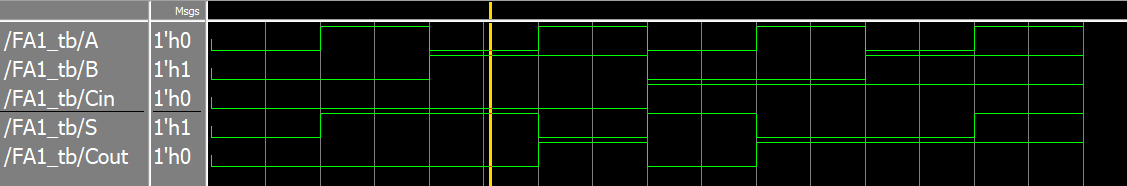
\includegraphics[width=\columnwidth]{FA_1B_sim}
		\caption{}
		\label{fig:fa1bsim}
	\end{figure}
	
	\subsection{Simulation results for the 2-bit full adder.}
	For the 2-bit full adder we then compare the results at the \(S\) and \(C_{out}\) output. On the Table \ref{tab:FA_2B_TT} the desired inputs and outputs are shown for a full adder, for the cases used.
	
	\begin{table}[H]
		\centering
		\begin{tabular}{|m{.2cm}|m{0.2cm}|m{0.5cm}|m{0.5cm}|}
			\hline
			\multicolumn{2}{|c|}{Inputs} & \multicolumn{2}{c|}{Outputs} \\
			\hline
			\(A\) & \(B\) & \(C_{out}\) & \(S\) \\
			\hline
			\centering\(00\) & \centering\(00\) & \centering\(0\) & \(00\) \\
			\centering\(01\) & \centering\(00\) & \centering\(0\) & \(01\) \\
			\centering\(00\) & \centering\(01\) & \centering\(0\) & \(01\) \\
			\centering\(01\) & \centering\(01\) & \centering\(0\) & \(10\) \\
			\centering\(10\) & \centering\(00\) & \centering\(0\) & \(10\) \\
			\centering\(11\) & \centering\(00\) & \centering\(0\) & \(11\) \\
			\centering\(11\) & \centering\(01\) & \centering\(1\) & \(00\) \\
			\centering\(11\) & \centering\(10\) & \centering\(1\) & \(01\) \\
			\centering\(11\) & \centering\(11\) & \centering\(1\) & \(10\) \\
			\hline
		\end{tabular}
		\caption{Truth table for a full adder.}
		\label{tab:FA_2B_TT}
	\end{table}
	
	The Figure \ref{fig:fa2bsim} shows the results of the simulation for the 2-bit full adder. And some of the cases of a full adder.
	
	\begin{figure}[H]
		\centering
		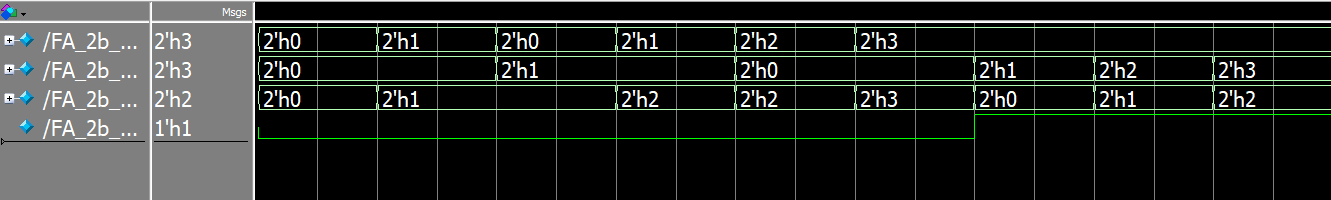
\includegraphics[width=0.9\columnwidth]{FA_2B_sim}
		\caption{}
		\label{fig:fa2bsim}
	\end{figure}
	
	\subsection{Simulation results for the 4-bit full adder.}
	
	For the 4-bit full adder we then compare the results we used all of the possible cases for the verification. On the Table \ref{tab:FA_4B_TT} the desired inputs and outputs are shown for a full adder, for the cases used.
	
	\begin{table}[H]
		\centering
		\begin{tabular}{|m{.2cm}|m{0.2cm}|m{0.5cm}|m{0.5cm}|}
			\hline
			\multicolumn{2}{|c|}{Inputs} & \multicolumn{2}{c|}{Outputs} \\
			\hline
			\(A\) & \(B\) & \(C_{out}\) & \(S\) \\
			\hline
			\centering\(00\) & \centering\(00\) & \centering\(0\) & \(00\) \\
			\centering\(01\) & \centering\(00\) & \centering\(0\) & \(01\) \\
			\centering\(00\) & \centering\(01\) & \centering\(0\) & \(01\) \\
			\centering\(01\) & \centering\(01\) & \centering\(0\) & \(10\) \\
			\centering\(10\) & \centering\(00\) & \centering\(0\) & \(10\) \\
			\centering\(11\) & \centering\(00\) & \centering\(0\) & \(11\) \\
			\centering\(11\) & \centering\(01\) & \centering\(1\) & \(00\) \\
			\centering\(11\) & \centering\(10\) & \centering\(1\) & \(01\) \\
			\centering\(11\) & \centering\(11\) & \centering\(1\) & \(10\) \\
			\hline
		\end{tabular}
		\caption{Truth table for a full adder.}
		\label{tab:FA_4B_TT}
	\end{table}
	
	The Figure \ref{fig:fa4bsim} shows the results of the simulation for the 4-bit full adder. And some of the cases of a full adder.
	
	\begin{figure}[H]
		\centering
		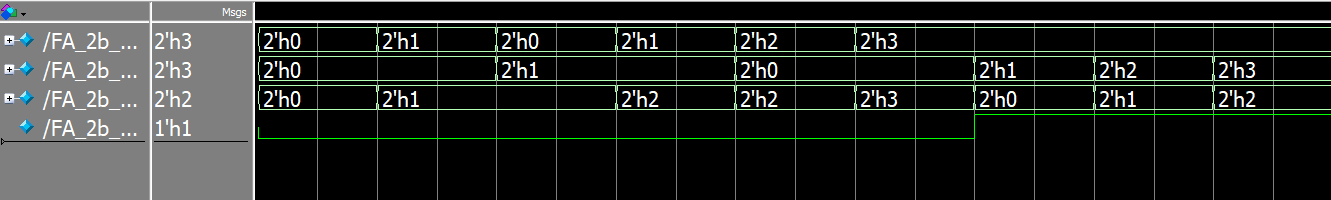
\includegraphics[width=0.9\columnwidth]{FA_2B_sim}
		\caption{}
		\label{fig:fa4bsim}
	\end{figure}
	
	\subsection{Simulation results for the 8-bit full adder.}
	
	For the 8-bit full adder we then compare the results we used all of the possible cases for the verification. On the Table \ref{tab:FA_8B_TT} the desired inputs and outputs are shown for a full adder, for the cases used.
	
	\begin{table}
		\centering
		\begin{tabular}{|m{1.2cm}|m{1.2cm}|m{0.5cm}|m{1.2cm}|}
			\hline
			\multicolumn{2}{|c|}{Inputs} & \multicolumn{2}{c|}{Outputs} \\
			\hline
			\(A\) & \(B\) & \(C_{out}\) & \(S\) \\
			\centering\(00000000\) & \centering\(00000000\) & \centering\(0\) & \(00000000\) \\ \hline
			\centering\(00000000\) & \centering\(00000000\) & \centering\(0\) & \(00000000\) \\ \hline
			\centering\(00000000\) & \centering\(00000001\) & \centering\(0\) & \(00000001\) \\ \hline
			\centering\(00000000\) & \centering\(00000001\) & \centering\(0\) & \(00000001\) \\ \hline
			\centering\(00000000\) & \centering\(00000010\) & \centering\(0\) & \(00000010\) \\ \hline
			\centering\(00000000\) & \centering\(00000010\) & \centering\(0\) & \(00000010\) \\ \hline
			\centering\(00000000\) & \centering\(00000011\) & \centering\(0\) & \(00000011\) \\ \hline
			\centering\(00000000\) & \centering\(00000011\) & \centering\(0\) & \(00000011\) \\ \hline
			\centering\(00000000\) & \centering\(00000100\) & \centering\(0\) & \(00000100\) \\ \hline
			\centering\(00000000\) & \centering\(00000100\) & \centering\(0\) & \(00000100\) \\ \hline
			\centering\(00000000\) & \centering\(00000101\) & \centering\(0\) & \(00000101\) \\ \hline
			\centering\(00000000\) & \centering\(00000101\) & \centering\(0\) & \(00000101\) \\ \hline
			\centering\(00000000\) & \centering\(00000110\) & \centering\(0\) & \(00000110\) \\ \hline
			\centering\(00000000\) & \centering\(00000110\) & \centering\(0\) & \(00000110\) \\ \hline
			\centering\(00000000\) & \centering\(00000111\) & \centering\(0\) & \(00000111\) \\ \hline
			\centering\(00000000\) & \centering\(00000111\) & \centering\(0\) & \(00000111\) \\ \hline
			\centering\(00000000\) & \centering\(00001000\) & \centering\(0\) & \(00001000\) \\ \hline
			
			\hline
		\end{tabular}
		\caption{Truth table for an 8 bit full adder.}
		\label{tab:FA_8B_TT}
	\end{table}
	
	The Figures \ref{fig:fa8bsim1} to \ref{fig:fa8bsim2} show some of the results of the simulation for the 8-bit full adder. And some of the cases of a full adder.
	
	\begin{figure}[H]
		\centering
		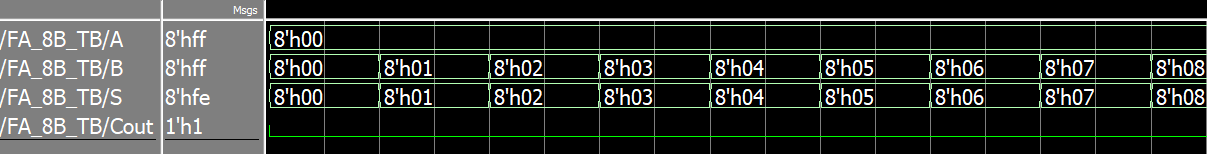
\includegraphics[width=0.9\columnwidth]{FA_8B_sim1}
		\caption{}
		\label{fig:fa8bsim1}
	\end{figure}
	
	\begin{figure}[H]
		\centering
		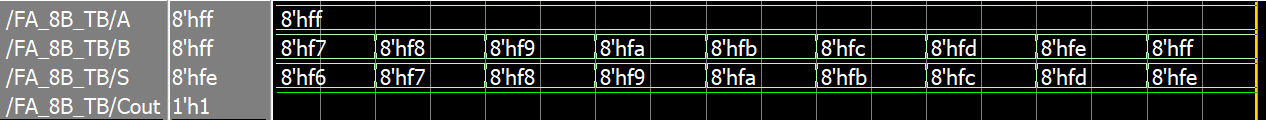
\includegraphics[width=0.9\columnwidth]{FA_8B_sim2}
		\caption{}
		\label{fig:fa8bsim2}
	\end{figure}
	
	
	\subsection{Simulation results for the 16-bit full adder.}
	
	For the 8-bit full adder we then compare the results we used all of the possible cases for the verification. On the Table \ref{tab:FA_16B_TT} the desired inputs and outputs are shown for a full adder, for the cases used.
	
	\begin{table}
		\centering
		\begin{tabular}{|m{1.2cm}|m{1.2cm}|m{0.5cm}|m{1.2cm}|}
			\hline
			\multicolumn{2}{|c|}{Inputs} & \multicolumn{2}{c|}{Outputs} \\
			\hline
			\(A\) & \(B\) & \(C_{out}\) & \(S\) \\
			\centering\(00000000\) & \centering\(00000000\) & \centering\(0\) & \(00000000\) \\ \hline
			\centering\(00000000\) & \centering\(00000000\) & \centering\(0\) & \(00000000\) \\ \hline
			\centering\(00000000\) & \centering\(00000001\) & \centering\(0\) & \(00000001\) \\ \hline
			\centering\(00000000\) & \centering\(00000001\) & \centering\(0\) & \(00000001\) \\ \hline
			\centering\(00000000\) & \centering\(00000010\) & \centering\(0\) & \(00000010\) \\ \hline
			\centering\(00000000\) & \centering\(00000010\) & \centering\(0\) & \(00000010\) \\ \hline
			\centering\(00000000\) & \centering\(00000011\) & \centering\(0\) & \(00000011\) \\ \hline
			\centering\(00000000\) & \centering\(00000011\) & \centering\(0\) & \(00000011\) \\ \hline
			\centering\(00000000\) & \centering\(00000100\) & \centering\(0\) & \(00000100\) \\ \hline
			\centering\(00000000\) & \centering\(00000100\) & \centering\(0\) & \(00000100\) \\ \hline
			\centering\(00000000\) & \centering\(00000101\) & \centering\(0\) & \(00000101\) \\ \hline
			\centering\(00000000\) & \centering\(00000101\) & \centering\(0\) & \(00000101\) \\ \hline
			\centering\(00000000\) & \centering\(00000110\) & \centering\(0\) & \(00000110\) \\ \hline
			\centering\(00000000\) & \centering\(00000110\) & \centering\(0\) & \(00000110\) \\ \hline
			\centering\(00000000\) & \centering\(00000111\) & \centering\(0\) & \(00000111\) \\ \hline
			\centering\(00000000\) & \centering\(00000111\) & \centering\(0\) & \(00000111\) \\ \hline
			\centering\(00000000\) & \centering\(00001000\) & \centering\(0\) & \(00001000\) \\ \hline
			
			\hline
		\end{tabular}
		\caption{Truth table for an 8 bit full adder.}
		\label{tab:FA_16B_TT}
	\end{table}
	
	The Figures \ref{fig:fa16bsim1} to \ref{fig:fa16bsim2} show some of the results of the simulation for the 8-bit full adder. And some of the cases of a full adder.
	
	\begin{figure}[H]
		\centering
		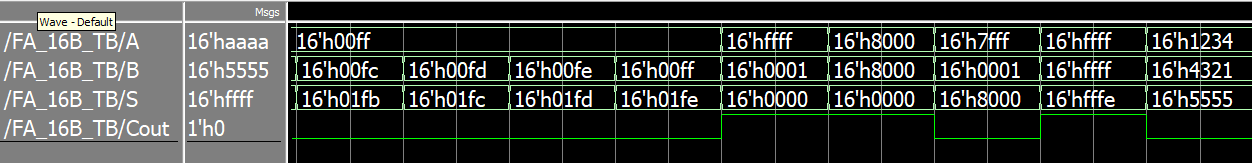
\includegraphics[width=0.9\columnwidth]{FA_16B_sim1}
		\caption{}
		\label{fig:fa16bsim1}
	\end{figure}
	
	\begin{figure}[H]
		\centering
		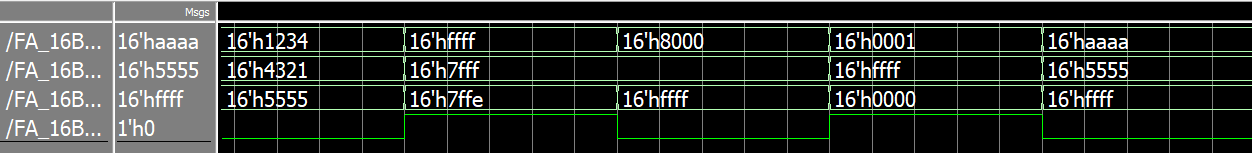
\includegraphics[width=0.9\columnwidth]{FA_16B_sim2}
		\caption{}
		\label{fig:fa16bsim2}
	\end{figure}
	
	
	
	
	
	
	
	\section{Conclusions}
	Throughout the development of this project, we successfully designed and tested a 16-bit full adder circuit. We also created code to generate test cases and fully implemented instances of simpler circuits to build more complex ones. We designed a test bench to verify various cases.
	
	
	\bibliographystyle{IEEEtran}
	%\bibliography{References}
	
	
	
	
	
	
\end{document}
